\section{Definition}
\vspace{0.2in}
\hspace*{0.16in}

A blood cell, also called a hematopoietic cell, hemocyte, or hematocyte, is a cell produced through hematopoiesis and found mainly in the blood. Major types of blood cells include red blood cells (erythrocytes), white blood cells (leukocytes), and platelets (thrombocytes). Together, these three kinds of blood cells add up to a total 45\% of the blood tissue by volume, with the remaining 55\% of the volume composed of plasma, the liquid component of blood. \textsuperscript{\cite{hopkins1993human}}\\

\vspace{0.1in}

\begin{figure}[h]
\centering
  \vspace{-0.1in}
    \centerline{\fbox{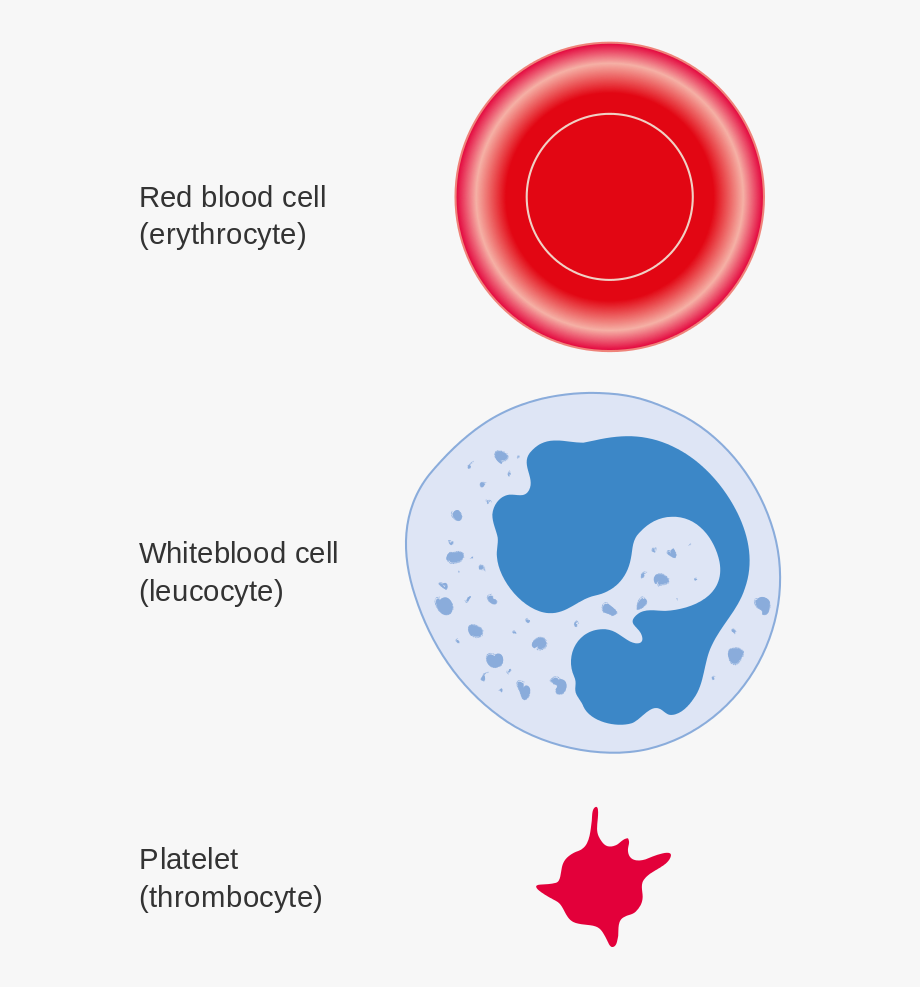
\includegraphics[width = 3in, height = 3in]{../images/blood_cells.png}}}
    \caption{Blood cells}
\end{figure}

That said, there are three main types of blood cells:

\subsection{Red blood cells}
\vspace{0.1in}
\hspace*{0.16in}


\subsection{White blood cells}
\vspace{0.1in}
\hspace*{0.16in}


\subsection{Platelets blood cells}
\vspace{0.1in}
\hspace*{0.16in}
